\section{Contouring and Isosurfaces}

\subsection{Contours}
Contours are a set of points where the scalar field $s$ has a given value $c$:
\begin{align*}
    \left\{ x\in \R^n: s(x) = c\right\}
\end{align*}

Examples in 2D:
\begin{itemize}
    \item Height contours on maps
    \item Isobars on weathermaps
\end{itemize}

\paragraph{Contouring algorithm:}
\begin{itemize}
    \item Find intersection with grid edges
    \item Connect points in each cell
\end{itemize}

\begin{figure}[H]
    \centering
    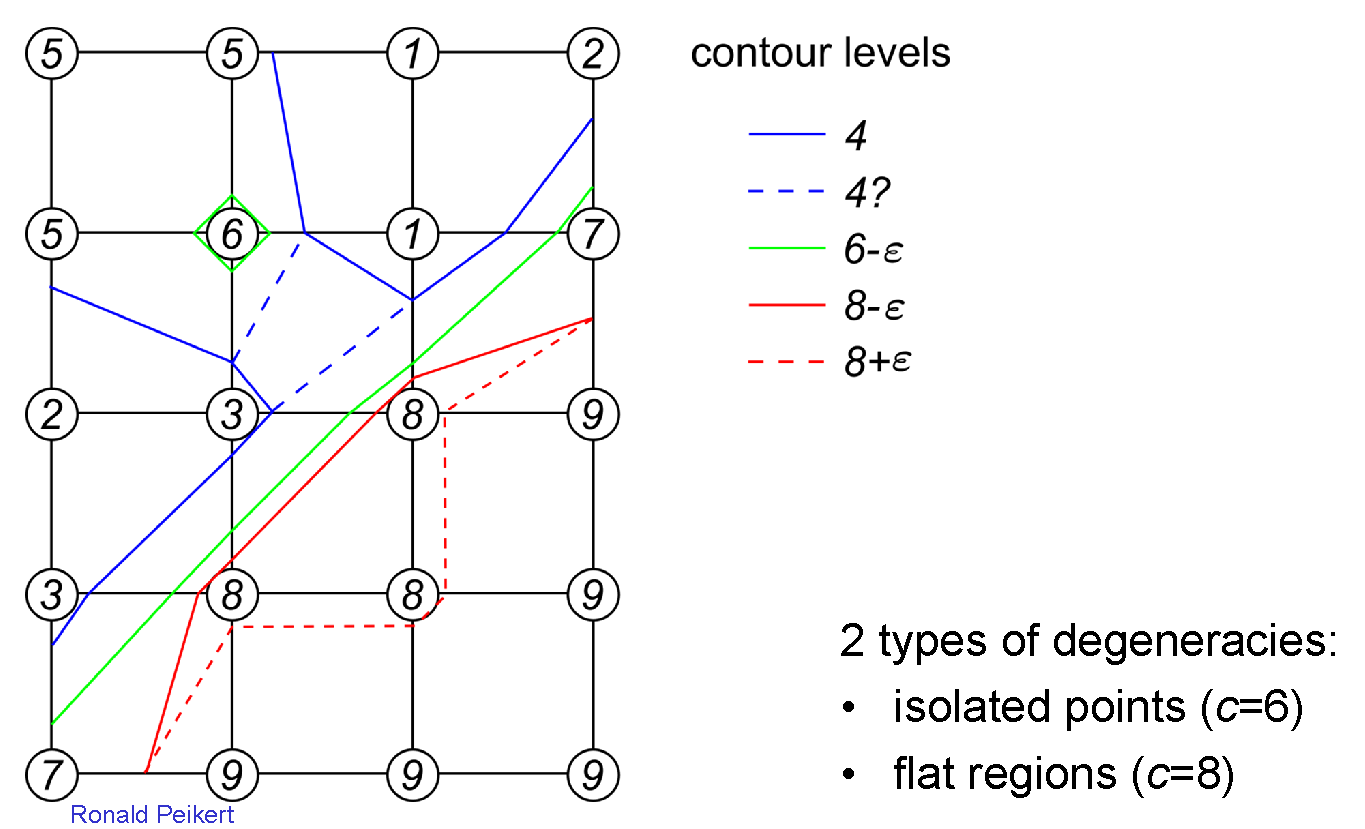
\includegraphics[width=0.75\textwidth]{img/02_contouring_example}
\end{figure}

\paragraph{Topological consistency}
To avoid degeneracies, use \emph{symbolic perturbations}:
\begin{description}
    \item If level $c$ is found as a node value, set the level to $c+\varepsilon$ where $\varepsilon$ is an infinitesimal, i.e., $\varepsilon >0$ and $\varepsilon < x$ $\forall x\in \R$.
\end{description}
Then:
\begin{itemize}
    \item Contours intersect edges at some (possibly infinitesimal) distance from end points.
    \item Flat regions can be visualised by a pair of contours at $c-\varepsilon$ and $c+\varepsilon$.
    \item Contours are \emph{topologically consistent}, meaning:\\
    
        Contours are \emph{closed}, \emph{orientable}, \emph{nonintersecting lines}.    
\end{itemize}

\paragraph{Ambiguities of contours} What is the \emph{correct} contour of $c=4$? 
\begin{figure}[H]
    \centering
    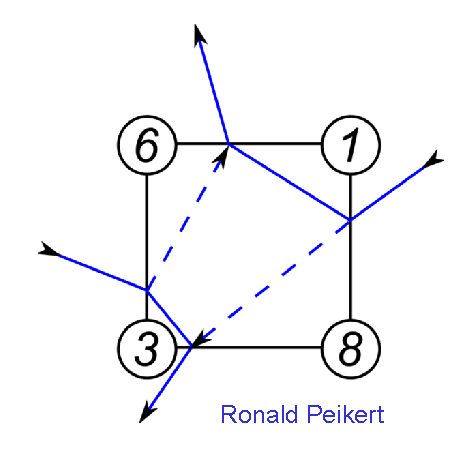
\includegraphics[width=0.3\textwidth]{img/02_contouring_c_4}
\end{figure}
Two possibilities (from which both are orientable):
\begin{itemize}
    \item Connecting the high values \rule{2cm}{0.9pt}
    \item Connecting the low values $- - - - - -$
\end{itemize}

\subsubsection{Contours in a quadrangle cell} 
\begin{description}
\item Local Coordinates $(0,0)\quad (1,0)\quad (0,1)\quad (1,1)$
\item Function Values $\quad s_{00}\quad s_{10}\quad s_{01}\quad s_{11}$
\item Bilinear Interpolant 
    \begin{align*}
     s(x,y) &= (1-x)(1-y)\ s_{00} + x(1-y) \ s_{10}+(1-x)y\ s_{01} + xy\ s_{11}\\
       &= Axy + Bx + Cy + D\\
       \text{with }\quad A &= s_{11}-s_{01}-s_{10}-s_{00}\\
       B &= s_{10}-s_{00}\\
       C &= s_{01}-s_{00}\\
       D &= s_{00}
    \end{align*}
\end{description}

\begin{itemize}
    \item If $A=0$, then the contour equation is $c=Bx+Cy+D$ and the contours are \emph{straight lines}, all parallel.
    \item If $A\neq 0$, then the contour equation is 
        \begin{align*}
            c = A\left( x+{C\over A}\right) (y+{B\over A})+D-{BC\over A}
        \end{align*}
        and the contours are \emph{hyperbola} except for the level
        \begin{align*}
            c = D- {BC\over A}.
        \end{align*}
        
        
        For the special level the contour equation is
            \begin{align*}
                0 = A\left( x+{C\over A}\right) \left( y+{B\over A}\right),
            \end{align*}
        and the contour is a pair of axis-aligned straight lines with
        \begin{align*}
            x &= -{C\over A},\\
            y &= -{B\over A}.
        \end{align*}
\end{itemize}

Decision can be made without computing special level or saddle points by just comparing fractions of edges:
\begin{figure}[H]
    \centering
    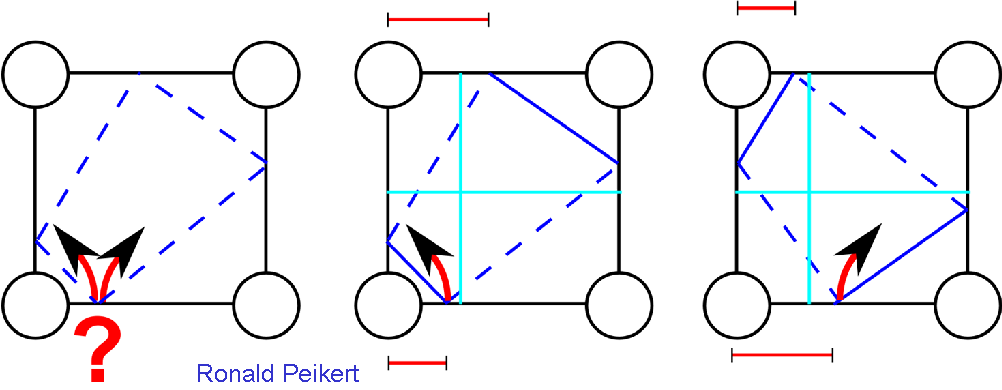
\includegraphics[width=0.75\textwidth]{img/02_contouring_decision}
\end{figure}
By using local coordinates, this works also for curvilinear and unstructured grids.

Not that drawing hyperbola instead of straight lines does not lead to better contours: The piecewise bilinear function is not in $C^1$.

\subsubsection{Basic contouring algorithms}
\begin{description}
    \item[Cell-By-Cell algorithms:] Simple structure, but generate disconnected segments and require post-processing.
    \item[Contour Propagation methods:] Complicated, but generate connected contours.
    \item[Marching Squares algorithm:] Systematic cell-by-cell algorithm. (See below)
\end{description}

\subsubsection{Marching Squares}
Process nodes in ccw (counter-clockwise order), denoted here as $x_0$, $x_1$, $x_2$ and $x_3$. At each node $x_i$ compute the reduced field
\begin{align*}
    \tilde s (x_i) &= s(x_i) - (c-\varepsilon) &\text{(which is forced to be nonzero)}.
\end{align*}
Take it's signe as the $i^{th}$ bit of a $4$-bit integer. Use this as an index for the lookup table containing the connectivity information.
\begin{figure}[H]
    \centering
    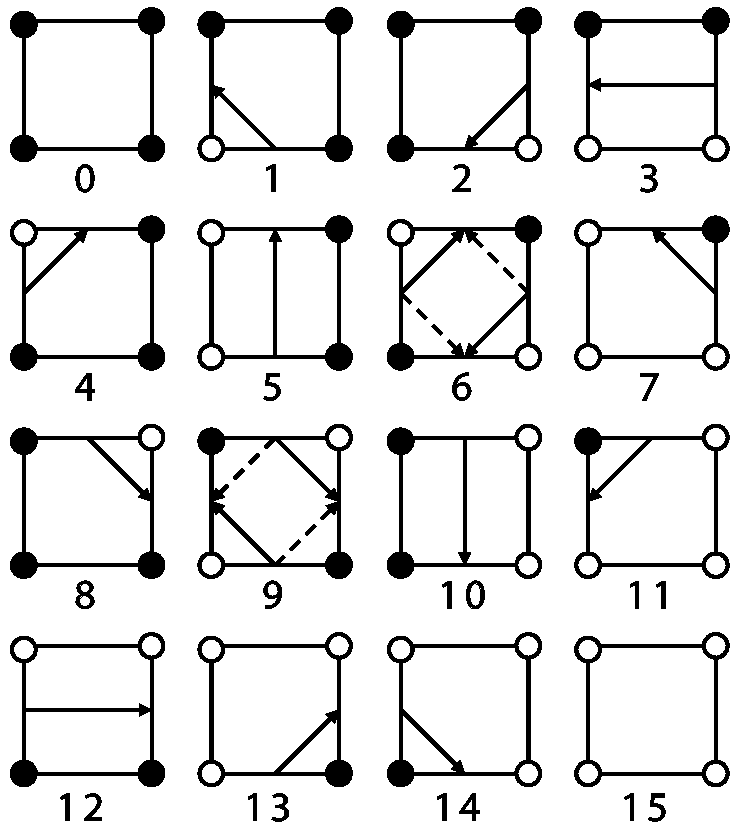
\includegraphics[width=0.5\textwidth]{img/02_marching_squares}
\end{figure}
\begin{align*}
   \bullet\quad \tilde s(x_i) &<0\\
   \circ\quad \tilde s(x_i) &>0
\end{align*}

Alternating signs exist in cases $6$ and $9$. Chose the solid or the dashed line based on topological \emph{consitency}.

\paragraph{Contours in triangle/tetrahedral cells} Linear interpolation of cells implies piece-wise linear contours. Since contours are unambiguous let us introduce a "marching triangles" method. This however introduces periodic artefacts.

\subsection{The Marching Cubes Algorithm}
Contours of $3$D scalar fields are known as \emph{isosurfaces}. Before 1987, isosurfaces were computed as contours on planar \emph{slices}, followed by "contour stitching".

The \emph{marching cubes} algorithm computes contours \emph{directly in 3D}:
\begin{itemize}
    \item Pieces of the isosurfaces are generated on a cell-by-cell basis.
    \item Similar to marching squares, an $8$-bit number is computed from the $8$ signs of $\tilde s(x_i)$ on the corners of a hexahedral cell.
    \item The isosurface piece is looked up in a table with $256$ entries.
\end{itemize}

How to build up the table of $256$ cases?

Lorensen and Cline (1987) exploited $3$ types of symmetries:
\begin{itemize}
    \item Rotational symmetries of the cube
    \item Reflective symmetries of the cube
    \item Sign changes of $\tilde s(x)$.
\end{itemize}

They published a reduced set of $14$ cases:
\begin{itemize}
    \item White circle indicate positive signs of $\tilde s(x)$ ,
    \item The positive side of the isosurface is drawn in red, the negative side in blue.
\end{itemize}

\begin{figure}[H]
    \centering
    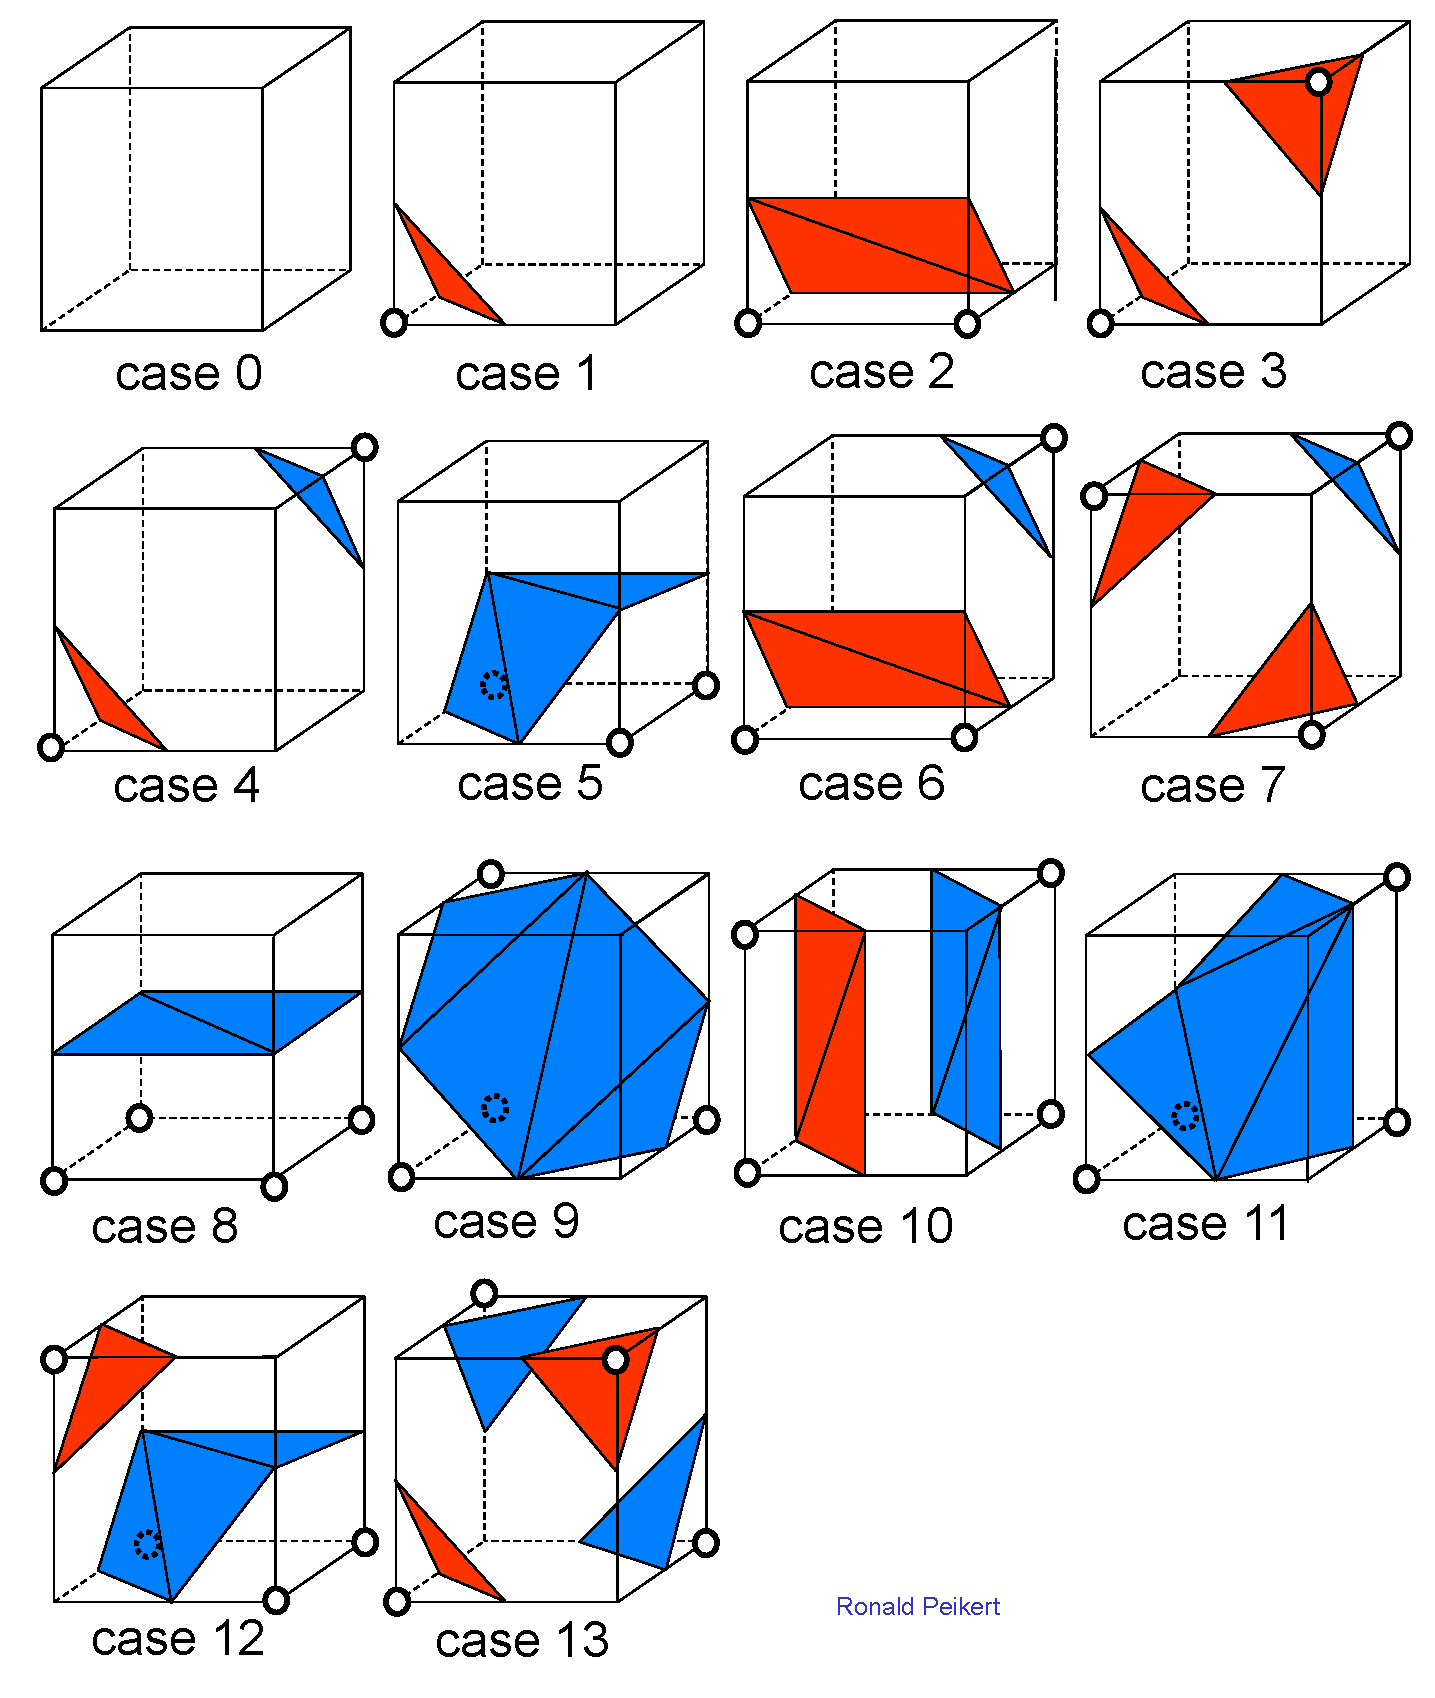
\includegraphics[width=0.75\textwidth]{img/02_marching_cubes}
\end{figure}

Unfortunately not all pieces fit together (same problem as with marching squares) and additional cases need to be introduced. 
\begin{figure}[H]
    \centering
    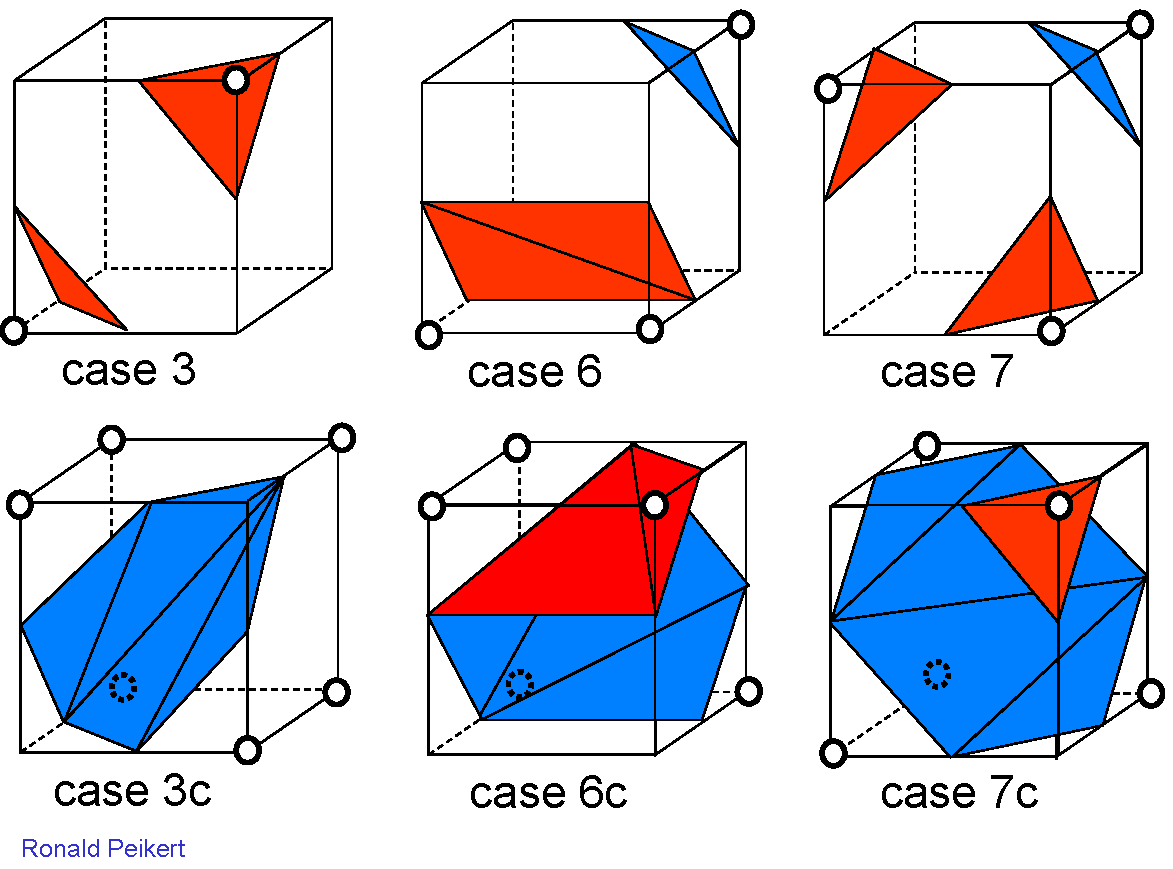
\includegraphics[width=0.75\textwidth]{img/02_marching_cubes_additional_cases}
\end{figure}

The remaining complementary cases are simply obtained by changing the the orientation. Based on these $28$ cases, the full $256$ cases are obtained by rotations of the cube.

\paragraph{Summary} of the algorithm:
\begin{enumerate}
    \item Pre-processing:
        \begin{itemize}
            \item Build a table of the $28$ cases.
            \item Derive a table of the $256$ cases, containing info on
            \begin{itemize}
                \item Intersected cell edges
                \item Triangles based on these points
            \end{itemize}
        \end{itemize}
    \item Loop over cells:
        \begin{itemize}
            \item Find sign of $\tilde s(x)$ for the $8$ corner nodes, giving $8$-bit integer.
            \item Use as index into lookup table.
            \item Find intersection points on edges listed in table, use linear interpolation.
            \item Generated triangles according to table.
        \end{itemize}
    \item Post-processing steps:
        \begin{itemize}
            \item Connect triangles (share vertices)
            \item Compute normal vectors:
                \begin{itemize}
                    \item By averaging triangle normals (problem: thin triangles!).
                    \item By estimating the gradient of the field $s(x)$ (better).
                \end{itemize}
        \end{itemize}
\end{enumerate}

\subsection{The Asymptotic Decider Algorithm}
Motivation for a different isosurface algorithm: Marching cubes can produce "bad" topology.

\emph{Asymptotic decider} algorithm (Nielson and Hamann 1991):
\begin{itemize}
    \item Generate topologically \emph{correct} contours (as oriented straight line segments) on the cell surfaces.
    \item Connect these around the cell, resulting in one or more polygons.
    \item Triangulate the polygons.
\end{itemize}
In general, the AD algorithm generates better isosurfaces. However,
\begin{itemize}
    \item It cannot be easily implemented with a table like Marching Cubes (too many cases).
    \item It generates polygons with up to $12$ sides (Marching Cubes: up to 7).
    \item The topology is correct with respect to the trilinear interpolant, but the geometry can deviate.
    \item Some polygons cannot be "cleanly" triangulated.
\end{itemize}

\subsection{The Dividing Cubes Algorithm}
An early \emph{point-based} algorithm (Crawford et al. '87): For each cell
\begin{itemize}
    \item Check whether it is intersected by the isosurface:
        \begin{align*}
            \min_{i\in \text{cell}} s_i < c < \max_{i\in \text{cell}} s_i
        \end{align*}
    \item Subdivide the intersected cell into $m\times m\times m$ subcells using trilinear interpolation.
    \item Draw the centers of all intersected subcells.
    \item To light the points estimate the gradient and use it as the normal vector.
\end{itemize}

\subsection{Optimised Isosurface Algorithms}
Approaches to speeding up isosurface computation:
\begin{description}
\item[View Dependent] algorithms:
    \begin{itemize}
        \item Occluded triangles are not computed
        \item GPU-based isosurface computation and redenring
    \end{itemize}
\item[Data Processing] for fast computation of \emph{multiple} isosurfaces (multiple levels), for example for interactive exploration of the data.
    \begin{itemize}
        \item Many methods: Octree, Extrema Graph, Span Space.
        \item Common Goal: Avoid computation in non-intersected cells.
    \end{itemize}
\end{description}

\subsubsection{The Span-Space Algorithm}
Method by Livnat (1996).
\begin{enumerate}
\item Pre-Processing. For each element
    \begin{itemize}
        \item Compute $\min$ and $\max$ ,
        \item Treat $(\min,\max)$ as a point in the \emph{span space} (Euclidean plane).
        \item Store points in boxes, non-empty boxes are stored in a linked list.
    \end{itemize}
\item Computation of the isosurface level $c$:

    Find the intersected cells in the \emph{quadrant} $\min < c$, $\max > c$.
    \begin{figure}[H]
    \centering
        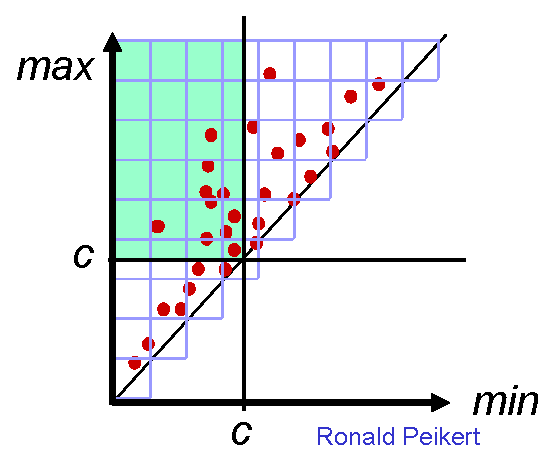
\includegraphics[width=0.5\textwidth]{img/02_span_space_algorithm}    
        \caption{Node distribution in span space.}
    \end{figure}

\end{enumerate}

This algorithm yields a performance gain for datasets with a small local variation, i.e. points in the span space are distributed on the diagonal.

\subsection{Selecting Contour Levels}
Several types of isosurface statistics can help with level selection. 
\begin{figure}[H]
\centering
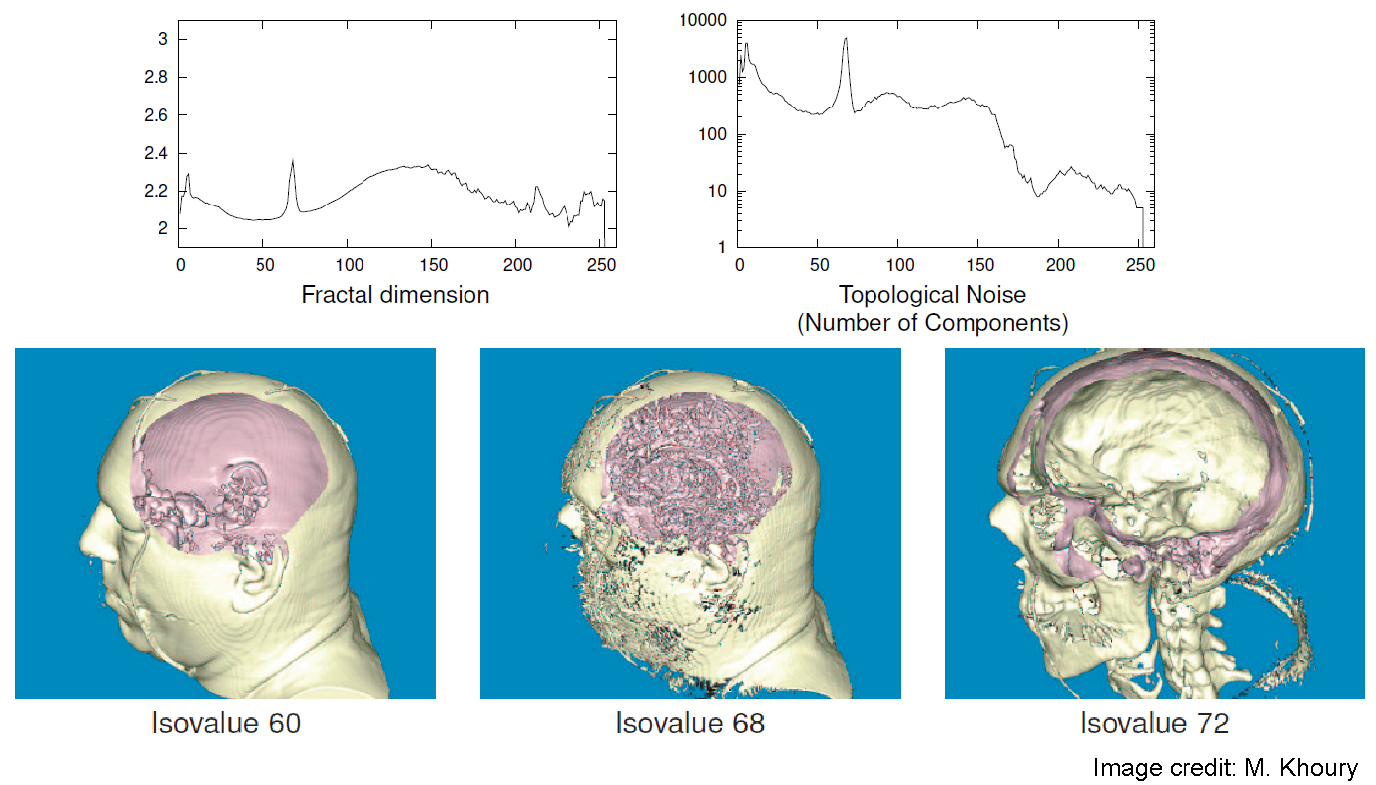
\includegraphics[width=0.9\textwidth]{img/02_contouring_statistics}
\end{figure}

\subsection{Limitations of Isosurfaces}
Isosurfaces represent only a single level within the data range. In practical data, there is often not a single "interesting" level.

Transparent rendering of multiple isosurfaces is possible, but
\begin{itemize}
    \item Limited to a small number of surfaces by visibility
    \item Alpha-blending require depth sorting.
\end{itemize}

Alternatives:
\begin{itemize}
    \item \emph{Feature Extraction methods}, e.g. detecting "blobs" (maximal ellipse-like contours)
    \item \emph{Volume rendering} can show ranges of "interesting levels of the field and/or its gradient.
\end{itemize}







